%%%%%%%%%%%%%%%%%%%%%%%%%%%%%%%%%%%%%%%%%
% Beamer Presentation
% LaTeX Template
% Version 1.0 (10/11/12)
%
% This template has been downloaded from:
% http://www.LaTeXTemplates.com
%
% License:
% CC BY-NC-SA 3.0 (http://creativecommons.org/licenses/by-nc-sa/3.0/)
%
%%%%%%%%%%%%%%%%%%%%%%%%%%%%%%%%%%%%%%%%%

%----------------------------------------------------------------------------------------
%	PACKAGES AND THEMES
%----------------------------------------------------------------------------------------

\documentclass[10pt,xcolor={usenames,dvipsnames,svgnames,table}]{beamer}

\mode<presentation> {

% The Beamer class comes with a number of default slide themes
% which change the colors and layouts of slides. Below this is a list
% of all the themes, uncomment each in turn to see what they look like.

%\usetheme{default}
%\usetheme{AnnArbor}
%\usetheme{Antibes}
%\usetheme{Bergen}
%\usetheme{Berkeley}
%\usetheme{Berlin}
%\usetheme{Boadilla}
%\usetheme{CambridgeUS}
%\usetheme{Copenhagen}
%\usetheme{Darmstadt}
%\usetheme{Dresden}
%\usetheme{Frankfurt}
\usetheme{Goettingen}
%\usetheme{Hannover}
%\usetheme{Ilmenau}
%\usetheme{JuanLesPins}
%\usetheme{Luebeck}
%\usetheme{Madrid}
%\usetheme{Malmoe}
%\usetheme{Marburg}
%\usetheme{Montpellier}
%\usetheme{PaloAlto}
%\usetheme{Pittsburgh}
%\usetheme{Rochester}
%\usetheme{Singapore}
%\usetheme{Szeged}
%\usetheme{Warsaw}

% As well as themes, the Beamer class has a number of color themes
% for any slide theme. Uncomment each of these in turn to see how it
% changes the colors of your current slide theme.

%\usecolortheme{albatross}
%\usecolortheme{beaver}
%\usecolortheme{beetle}
%\usecolortheme{crane}
%\usecolortheme{dolphin}
%\usecolortheme{dove}
%\usecolortheme{fly}
%\usecolortheme{lily}
%\usecolortheme{orchid}
%\usecolortheme{rose}
\usecolortheme{seagull}
%\usecolortheme{seahorse}
%\usecolortheme{whale}
%\usecolortheme{wolverine}

%\setbeamertemplate{footline} % To remove the footer line in all slides uncomment this line
\setbeamertemplate{footline}[text line]{Test} % To replace the footer line in all slides with a simple slide count uncomment this line

\setbeamertemplate{navigation symbols}{} % To remove the navigation symbols from the bottom of all slides uncomment this line
}

\usepackage{graphicx} % Allows including images
\usepackage{booktabs} % Allows the use of \toprule, \midrule and \bottomrule in tables
\usepackage[ngerman]{babel} 
\usepackage[utf8]{inputenc}
\usepackage{hyperref}

\newcommand\blfootnote[1]{%
  \begingroup
  \renewcommand\thefootnote{}\footnote{#1}%
  \addtocounter{footnote}{-1}%
  \endgroup
}

%----------------------------------------------------------------------------------------
%	TITLE PAGE
%----------------------------------------------------------------------------------------

\title[]{Clustern von Relationen zwischen Wortvektoren\footnote{Arbeitstitel}} % The short title appears at the bottom of every slide, the full title is only on the title page

\author{\textsc{Dennis Ulmer}} % Your name
\institute[Institut für Computerlinguistik]{
	Computerlinguistisches Abschlusskolloquium\\
	Insitut für Computerlinguistik
} % Your institution as it will appear on the bottom of every slide, may be shorthand to save space
\date{15. Dezember 2015} % Date, can be changed to a custom date

\defbeamertemplate*{footline}{mytheme}
{
  \leavevmode%
  \hbox{%
  \begin{beamercolorbox}[wd=.55\paperwidth,ht=2.25ex,dp=1ex,center]{author in head/foot}%
    \usebeamerfont{author in head/foot}\insertshortauthor
  \end{beamercolorbox}%
  \begin{beamercolorbox}[wd=.45\paperwidth,ht=2.25ex,dp=1ex,right]{date in head/foot}%
    \usebeamerfont{date in head/foot}\insertshortdate{}\hspace*{2em}
    \insertframenumber{} / \inserttotalframenumber\hspace*{2ex} 
  \end{beamercolorbox}}%
  \vskip0pt%
}
\usebeamertemplate{mytheme}

\begin{document}

\begin{frame}
	\titlepage
\end{frame}

\begin{frame}
	\frametitle{Gliederung} % Table of contents slide, comment this block out to remove it
	\setcounter{tocdepth}{2}
	\tableofcontents % Throughout your presentation, if you choose to use \section{} and \subsection{} commands, these will automatically be printed on this slide as an overview of your presentation
\end{frame}

\begin{frame}
	\section{Distributionelle Semantik}
	\frametitle{Distributionelle Semantik \& Knowledge Graph Completion} 
	\begin{block}{Distributional hypothesis}
		Words that occur in the same contexts tend to have similar meanings (Harris 1954)
	\end{block}
	\begin{itemize}
		\item[$\hookrightarrow$] Trainieren von Wortvektoren ($\rightarrow$ \texttt{word2vec})
		\item $vector(King) - vector(Man) + vector(Woman) \approx vector(Queen)$
	\end{itemize} 
\end{frame}

\begin{frame}
	\frametitle{Knowledge Graph Completion}
	\begin{block}{Knowledge Graph Completion}
		``Knowledge graphs encode structured information of entities and their rich relations. [...] [A] typical knowledge graph [...] is usually far from complete. \textbf{Knowledge graph completion} aims at predicting relations between entities under supervision of the existing knowledge graph'' (Lin et al. 2015)
	\end{block}
	$\hookrightarrow$ In semantischen Vektorraummodellen manifestieren sich manche Relationen durch einen ähnlichen Vektor zwischen Wortpaaren ($\rightarrow$ TransE)
\end{frame}

\begin{frame}
	\section{Idee}
	\frametitle{Idee}
	\begin{itemize}
		\item[$\rightarrow$] Trainieren von 1:1-, 1:N-, N:1- und N:N-Relationen in einem semantischen Vektorraum (Lin et al. 2015)
		\item[$\rightarrow$] Auffinden von Relationen innerhalb des Vektorraums fürs Deutsche (diese Bachelorarbeit!)
	\end{itemize}
\end{frame}

\begin{frame}
	\section{TransE, TransH, TransR, CTransR}
	\frametitle{TransE}
	\begin{itemize}
		\item Wortvektoren $h, t \in \mathbb{R}^k$
		\item Relationstripel: $(h, r, t)$, sodass $h + r \approx t$
		\item Kostenfunktion: $f_r(h, t) = \|h + r - t\|^2_2$
		\item[$\rightarrow$] Probleme: Modellieren von \emph{1:N}-, \emph{N:1}- und \emph{N:N}-Relationen
	\end{itemize}
	\begin{center}
		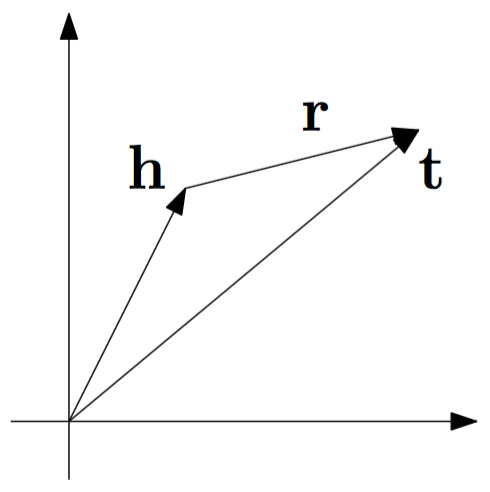
\includegraphics[scale=0.20]{./img/transe.png}
	\end{center}
\end{frame}

\begin{frame}
	\frametitle{TransH (Wang et al. 2014)}
	\begin{itemize}
		\item Idee: Projektion der Wortvektoren auf relationsspezifische Ebene, um alle Arten von Relationen modellieren zu können
		\item Projektion von $h$ und $t$ mit Normalvektor $w_r$ mit $\|w_r\|_2=1$:
		\item[] $h_\bot = h - w_r^\top hw_r$
		\item[] $t_\bot = t - w_r^\top tw_r$
		\item $f_r(h, t) = \|h_\bot + r + t_\bot\|^2_2$
		\item[$\rightarrow$ ] Probleme: Verschiedene (für Relationen wichige) Aspekte von Entitäten im Vektorraum werden nicht unterschieden
	\end{itemize}
	\begin{center}
		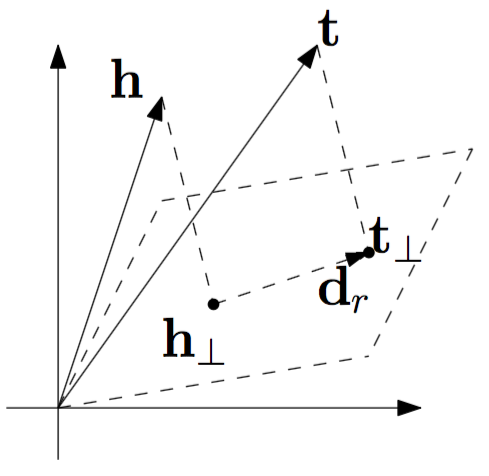
\includegraphics[scale=0.20]{./img/transh.png}
	\end{center}
\end{frame}

\begin{frame}
	\frametitle{TransR}
	\begin{itemize}
		\item Idee: Trennung von Entitäts- und Relationsraum
		\item Relationstripel $(h, r, t)$ mit $h, t \in \mathbb{R}^k$ und $r \in \mathbb{R}^d$, wobei $k \neq d$ sein kann
		\item Projektionsmatrix für jede Relation $M_r \in \mathbb{R}^{d\times k}$:
		\item[] $h_r = hM_r; t_r = tM_r$ 
		\item (Alte) Kostenfunktion $f_r(h, t) = \|h_r + r - t_r\|$
	\end{itemize}
	\begin{center}
		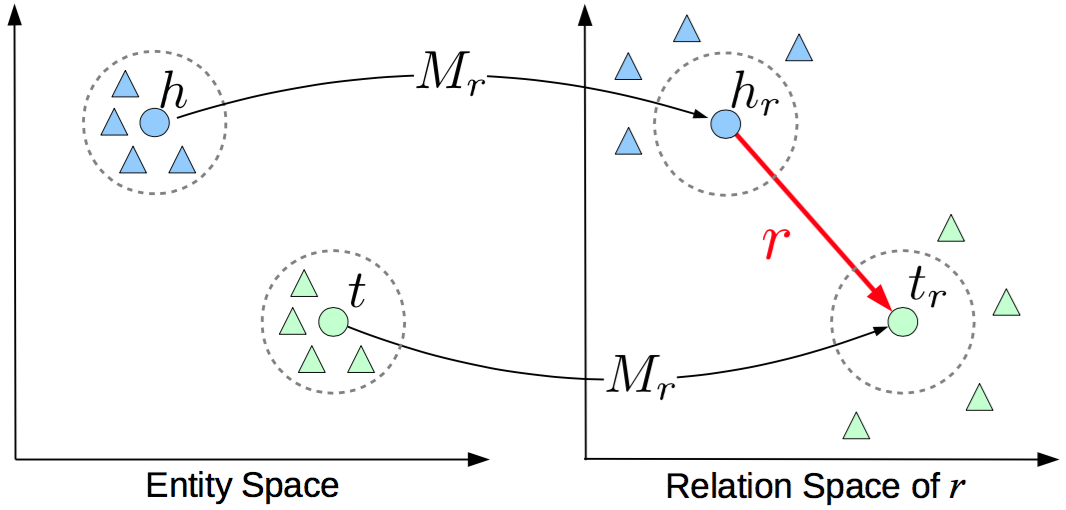
\includegraphics[scale=0.20]{./img/transr.png}
	\end{center}
\end{frame}

\begin{frame}
	\frametitle{Cluster-based Trans-R (CTransR)}
	\begin{itemize}
		\item[$\rightarrow$] Problem: Eine Relation wird verschiedenen ``Lesarten'' nicht gerecht
		\item Idee: Entitäten einer Relation nach Versatz $(h-t)$ clustern
		\item Danach: TransR mit clusterspezifischem $r_c$ trainieren
		\item $f_r(h, t) = \|h_{r, c} + r_c - t_{r,c}\|^2_2 + \alpha\|r_c-r\|^2_2$
	\end{itemize}
\end{frame}

\begin{frame}
	\section{Diese Arbeit}
	\frametitle{Diese Arbeit}
	\begin{itemize}
		\item Nicht alle Typen von Relationen funktionieren in einem semantischen Vektorraum
		\item[$\rightarrow$ ] Menschliche Vorauswahl (mit menschlichem Bias!)
		\item Idee: Entitätspaare nach Versatz (und anderen Features) clustern und Cluster auf Zugehörigkeit zu Relation prüfen
		\begin{itemize}
			\item Input: Deutsche Wortvektoren
			\item Output: Cluster aus Wortpaaren, die einem Relationstypen zuzuschreiben sind
		\end{itemize}
	\end{itemize}
\end{frame}

\begin{frame}
	\frametitle{Hypothese}
	\subsection{Hypothese}
	\begin{itemize}
		\item Trennung von Entitäts- und Relationsraum (hier allerdings nur \textbf{ein} Relationsraum)
		\item Wortpaar $(h, t)$, z.B. $(Paris, Frankreich)$ oder $(Paris, Blumentopf)$
		\item Mapping des Wortpaares in den Relationsraum:
		\item[] $\phi(h, t) \mapsto \tilde{r}_{h, t}$
		\item[] $h, t \in \mathbb{R}^k, \tilde{r}_{h, t} \in \mathbb{R}^d$, wieder $k \neq d$ möglich
	\end{itemize}
		\begin{block}{Hypothese}
			Cluster aus nahe beieinanderliegende $\tilde{r}_{h, t}$ gehören zu einer Relation
		\end{block}
\end{frame}

\begin{frame}
	\begin{itemize}
		\item Anspruch an $\phi(\cdot, \cdot)$: Zu einer Relation gehörenden Wortpaare sollten im Relationsraum möglichst nahe beieinander landen
		\item Mögliche Features für Mappingfunktion $\phi(\cdot, \cdot)$:
		\begin{itemize}
			\item Richtung \footnote{$\tilde{r}_{h, t} = t - h$ (= TransE!)}
			\item Länge
			\item ...
		\end{itemize}
		\item[$\rightarrow$] Offene Fagen:
		\begin{itemize}
			\item Welche Features für $\phi(\cdot, \cdot)$ übernehmen?
			\item Welche Features funktionieren? Welche nicht?
			\item (Wie TransE) \emph{1:N}-, \emph{N:1}- und \emph{N:N}-Relationen?
		\end{itemize}
	\end{itemize}
\end{frame}

% Ressourcen

	\begin{frame}
		\subsection{Ressourcen}
		\subsubsection{Decow-Korpus}
		\frametitle{Decow-Korpus}
		\begin{itemize}
			\item[=] \textbf{DE} \textbf{co}rpus from the \textbf{w}eb  
			\item Texte von deutschsprachigen Internetseiten
			\item Annotation mit PoS-, NE-Tags sowie Morphologie und Lemmata
			\item Außerdem: Diverse Meta-Informationen zu einzelnen Sätzen
			\item 21 Teile mit insgesamt $>$ 11,5 Mrd. Tokens in $>$ 600 Mio. Sätzen
		\end{itemize}
	\end{frame}

	\begin{frame}
		\subsubsection{Freebase}
		\frametitle{Freebase}
		\begin{center}
			
\includegraphics[scale=0.70]{./img/freebase.png}
		\end{center}
		\begin{itemize}
			\item Von Community gepflegte Graphbasierte Datenbank $\rightarrow$ Entitäten sind Knoten, Relationen sind Kanten
			\item In mehreren Sprachen verfügbar, durch Google API und Abfragesprache MQL abfragbar
			\item Aus Freebase: FB40K-Datenset (335.350 englische Relationstripel mit NEs)
		\end{itemize}n
	\end{frame}

	\begin{frame}
		\subsubsection{word2vec}
		\frametitle{word2vec}
		\begin{center}
			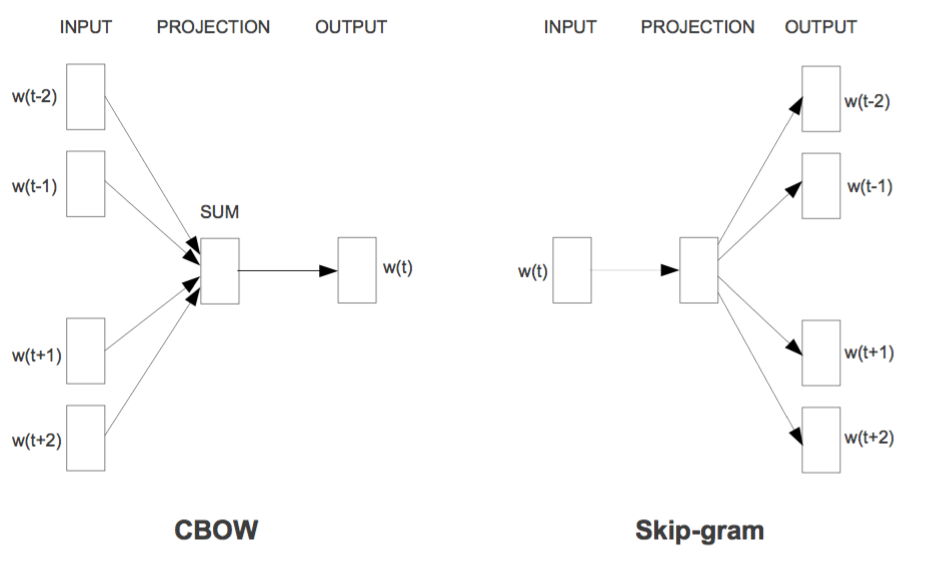
\includegraphics[height=0.4\paperheight, width=0.75\textwidth]{./img/cbow_skipgram.png}
		\end{center}
		\begin{itemize}
			\item C-Tool zum Trainieren von Wortvektoren (\emph{Word embeddings})
			\item Parameter:
			\begin{itemize}
				\item Skip-gram- oder Bag-of-words-Ansatz
				\item Lernalgorithmus
				\item Dimensionalität
				\item Größe des Kontextfensters
				\item Subsampling häufiger Wörter
				\item $\ldots$
			\end{itemize}
			\item[$\rightarrow$] Optimierung der Parameter auf Korpusausschnitt?
		\end{itemize}
	\end{frame}

\begin{frame}
	\subsection{Vorbereitungen}
	\frametitle{Vorbereitung}
	\begin{itemize}
		\item Deutsche Äquivalente für Relationsenden der FB40k-Daten abfragen (erfolgreich für $\sim$ 60 \%) $\rightarrow$ 204.016 deutsche Tripel
		\item Extrahieren aller NEs und ihrer Satz-IDs aus dem Decow-Korpus $\rightarrow$ $>$ 31 Mio. NEs
		\item Vorkommen von Mehrwort-NEs in Decow mit Unterstrich verbinden
		\item Trainieren der Wortvektoren 
		\item Extraktion von verwandten Entitäten zur Wortvektorevaluation ($\rightarrow$ ``Konzeptgruppen'')
	\end{itemize}
\end{frame}

\begin{frame}
	\subsection{Clustering}
	\frametitle{Clustering}
	\begin{itemize}
		\item Clustering der $\tilde{r}_{h, t}$ im Relationsraum nach räumlicher Nähe
		\item Clustering-Algorithmus verwenden, der die Anzahl der Cluster nicht von Anfang an vorgibt
		\item[$\rightarrow$] Offene Fragen: 
		\begin{itemize}
			\item Sinnvolle Einschränkungen für den Algorithmus?
			\item Welche Wortpaare machen überhaupt Sinn? $(Paris, Frankreich) \leftrightarrow (Paris, Blumentopf)$
		\end{itemize}
	\end{itemize}
\end{frame}

\begin{frame}
	\section{Evaluation}
	\frametitle{Evaluation}
	\begin{itemize}
		\item Daten aus Decow und FB40k
		\begin{itemize}
			\item Sind die ins deutsche übertragenen Daten aus FB40k fürs deutsche Relevant?
			\item[$\rightarrow$] Anteil von FB40k-NEs, die auch in Decow-NEs sind
			\item[$\rightarrow$] \textbf{88.954 \%}
		\end{itemize}
		\item Wortvektoren
		\begin{itemize}
			\item Haben die Wortvektoren überhaupt semantische Aussagekraft?
			\item[$\rightarrow$] Anteil von räumlich nahen Entitäten in Freebase-``Konzeptgruppen''
		\end{itemize}
		\item Geclusterte Relationen
		\begin{itemize}
			\item Wurden wirkliche Relationen gefunden?
			\item Einschränkung fürs erste auf NEs
			\item[$\rightarrow$] Anteil von Entitätspaaren in einem Cluster, die sich der gleichen Freebase-Relation zuordnen lassen
		\end{itemize}
	\end{itemize}
\end{frame}

\begin{frame}
	\section{Fahrplan}
	\frametitle{Fahrplan}
	\begin{itemize}
		\item Vorbereitungen \textcolor{Bittersweet}{$\ominus$}
		\begin{itemize}
			\item NEs in Decow extrahieren \textcolor{ForestGreen}{\checkmark}
			\item Deutsche FB40k-Tripel extrahieren \textcolor{ForestGreen}{\checkmark}
			\item[\textcolor{MidnightBlue}{\textbf{$\diamondsuit$}}] \textcolor{MidnightBlue}{\textbf{Evaluation: Relevanz von dt. FB40k-Tripeln}} \textcolor{ForestGreen}{\checkmark}
			\item Decow für Training vorbereiten \textcolor{Bittersweet}{$\ominus$}
			\item Konzeptgruppen aus Freebase extrahieren
			\item Wortvektoren trainieren \& Parameter optimieren
			\item[\textcolor{MidnightBlue}{\textbf{$\diamondsuit$}}] \textcolor{MidnightBlue}{\textbf{Evaluation: Wortvektoren}}
		\end{itemize}
		\item Mapping
		\begin{itemize}
			\item Verschiedene Mappingfunktionen $\phi(\cdot, \cdot)$ erstellen \& ausprobieren
		\end{itemize}
		\item Clustering
		\begin{itemize}
			\item Verschiedene Clusteralgorithmen ausprobieren
			\item[\textcolor{MidnightBlue}{\textbf{$\diamondsuit$}}] \textcolor{MidnightBlue}{\textbf{Evaluation: Gefundene Relationscluster}}
		\end{itemize}
	\end{itemize}
	\blfootnote{\textcolor{ForestGreen}{\checkmark}: Erledigt \hspace{0.25cm} \textcolor{Bittersweet}{$\ominus$}: In Arbeit}
\end{frame}

\begin{frame}
	\section{Quellen}
	\subsection{Literatur}
		\begin{itemize}
			\item \textsc{Harris, Zellig S.} ``Distributional structure.'' Word (1954).
			\item \textsc{Levy, Omer, Yoav Goldberg, and Ido Dagan.} ``Improving distributional similarity with lessons learned from word embeddings.'' Transactions of the Association for Computational Linguistics 3 (2015): 211-225.
			\item \textsc{Lin, Yankai, et al.} ``Learning entity and relation embeddings for knowledge graph completion.'' Proceedings of AAAI. 2015.
			\item \textsc{Mikolov, Tomas, Wen-tau Yih, and Geoffrey Zweig.} ``Linguistic Regularities in Continuous Space Word Representations.'' HLT-NAACL. 2013.
			\item \textsc{Wang, Zhen et al.} ``Knowledge graph embedding by translating on hyperplanes.'' Proceedings of the Twenty-Eighth AAAI Conference on Artificial Intelligence. 2014.
		\end{itemize}
	\frametitle{Literatur}
\end{frame}

\begin{frame}
	\subsection{Sonstiges}
		\begin{itemize}
			\item \texttt{word2vec.} Tool for computing continuous distributed representations of words. \url{https://code.google.com/p/word2vec/}
			\item \texttt{Freebase.} A community-curated database of well-known people, places, and things. \url{https://www.freebase.com}
		\end{itemize}
	\frametitle{Sonstiges}
\end{frame}


\end{document} 
